\chapter[Abordagem da Engenharia de Requisitos]{Abordagem da Engenharia de Requisitos}
A Engenharia de Requisitos (ER) é essencialmente um conjunto de atividades utilizadas para identificar e comunicar a finalidade de um sistema de software e o contexto no qual será usado. De acordo com Steve Easterbrook [\citeyear{easterbrook}], professor do Departamento de Ciência da Computação da Universidade de Toronto, a ER atua como a ponte entre as necessidades reais dos usuários, clientes, e outros grupos afetados por um sistema de software , e as potencialidades e oportunidades oferecidas pela tecnologia. 

Atualmente, observa-se uma necessidade de automatização de processos os quais são essenciais dentro de qualquer organização e em qualquer área de atuação, especialmente nas mais recentes, dentre as quais está inseria a produção de software. “A definiçãode processos de desenvolvimento de \textit{software} vem com o objetivo de aumentar a produtividade e diminuir os riscos de um projeto”~\cite{vieira}.

Um fator que deve ser levado em consideração na produção de \textit{software} é descrito como a produção de um produto intangível “construído estritamente por pessoas e totalmente suscetível a falhas”~\cite{tanenbaum}. Não obstante, a demanda recente do mercado por \textit{softwares} tem acarretado em um encurtamento substancial dos prazos para as entregas dos produtos e na contra mão dessa tendência há uma cobrança cada vez maior por qualidade. De acordo com Tavares [\citeyear{tavares}], a qualidade de um produto de \textit{software} está diretamente ligada a melhor forma de atender as necessidades do cliente, o que torna um produto totalmente dinâmico. Uma vez que a natureza do produto é dinâmica existem grandes dificuldades no gerenciamento do desenvolvimento, por exemplo: a essência volátil dos requisitos do cliente.

Dados estes fatores, atualmente existem vários modelos de processos dentro da Engenharia de Software, de forma que os riscos presentes no desenvolvimento sejam devidamente amenizados. Essas abordagens diminuem o tempo de produção e os recursos necessários para o desenvolvimento. Exemplo de processos são: cascata, interativo, espiral e incremental.

Cada processo se encaixa melhor em um determinado contexto, geralmente uma boa prática da ER é escolher e adaptar um modelo de processo de acordo com a equipe, com o cliente e com o projeto. Por conseguinte, levando-se em consideração principalmente o contexto do trabalho a ser confeccionado nessa disciplina foram propostas apenas duas abordagens, o Scaled Agile Framework e o Rational Unified Process. A seguir daremos uma breve explicação sobre como funciona cada uma das abordagens e em seguida será exposta a justificativa da escolha da abordagem e suas respectivas atividades.

  \section{SAFe}
Segundo Dean Leffingwell, representante da Scaled Agile, empresa que mantém O \textit{Scaled Agile Framework} (SAFe), este pode ser definido como uma base de conhecimento online e livre de padrões de sucesso comprovado para uma implementação ágil enxuta de empreendimentos em escala~\cite{deanleffingwell}.

A crença na qual o SAFe foi baseado gira em torno principalmente da satisfação do cliente. De acordo com o site do \textit{framework}, define-se a visão principal como \textit{“better systems and software make the world a better place”} - Melhores sistemas e \textit{softwares} fazem do mundo um lugar melhor.
Segundo dados da própria Scaled Agile, vários empreendimentos, de pequenos à grandes, estão reportando os benefícios da aplicação do SAFe. Entre eles estão:

\begin{itemize}
\item 20 - 50\% aumento na produtividade;
\item 50\%+ melhora da qualidade;
\item 30 - 75\% tempo de disponibilização para o mercado.
\item Aumento mensurável no envolvimento e satisfação dos funcionários;
\end{itemize}

Com esses resultados, o SAFe vem crescendo rapidamente por todo o mundo. A lista das 100 empresas mais relevantes da revista Fortune indica que 60\% delas tem certificado seus profissionais e consultores no processo.

Assim como o Scrum está para uma equipe ágil o SAFe está para um empreendimento ágil, possuindo uma abordagem focada na gestão e captura dos requisitos[IBM], em vez de no design e implementação.

É composto essencialmente por três níveis: o nível de Time, o nível de Programa e o nível de Portfólio. Para cada nível, existe um nível diferente de narrativa de requisitos: épicos para o Portfólio, features para o Programa e histórias de usuários para o Time. A partir da versão 4.0 deste framework, foi adicionado um novo nível, facultativo, chamado Fluxo de Valor.

O SAFe possui nove princípios fundamentais, baseados nos princípios ágeis, que orientam os papéis e práticas que o tornam efetivo. Esses princípios são:

\begin{itemize}
\item Tenha uma visão econômica
\item Tenha um pensamento sistêmico
\item Assuma variabilidade e preserve opções
\item Construa incrementalmente com ciclos de aprendizagem integrados e rápidos
\item Baseie os marcos em avaliação objetiva dos sistemas 	
\item Descentralize a tomada de decisão
\item Desbloqueie a motivação intrínseca aos profissionais do conhecimento
\item Tenha cadência; sincronize com planejamento cross-domain
\item Visualize e limite o trabalho em progresso, reduza a carga e gerencie o comprimento da fila
\end{itemize}

A Scaled Agile dá total suporte para a implementação do SAFe, possuindo centenas de consultores pelo mundo e disponibilizando vários artigos sobre como o processo de implementação pode ser colocado em prática. Um deles se chama \textit{Implementing 1-2-3} e pode ser encontrado em  www.scaledagileframework.com/implementing.

\subsection{Big picture do SAFe}
  \begin{figure}[!htbp]
    \centering
    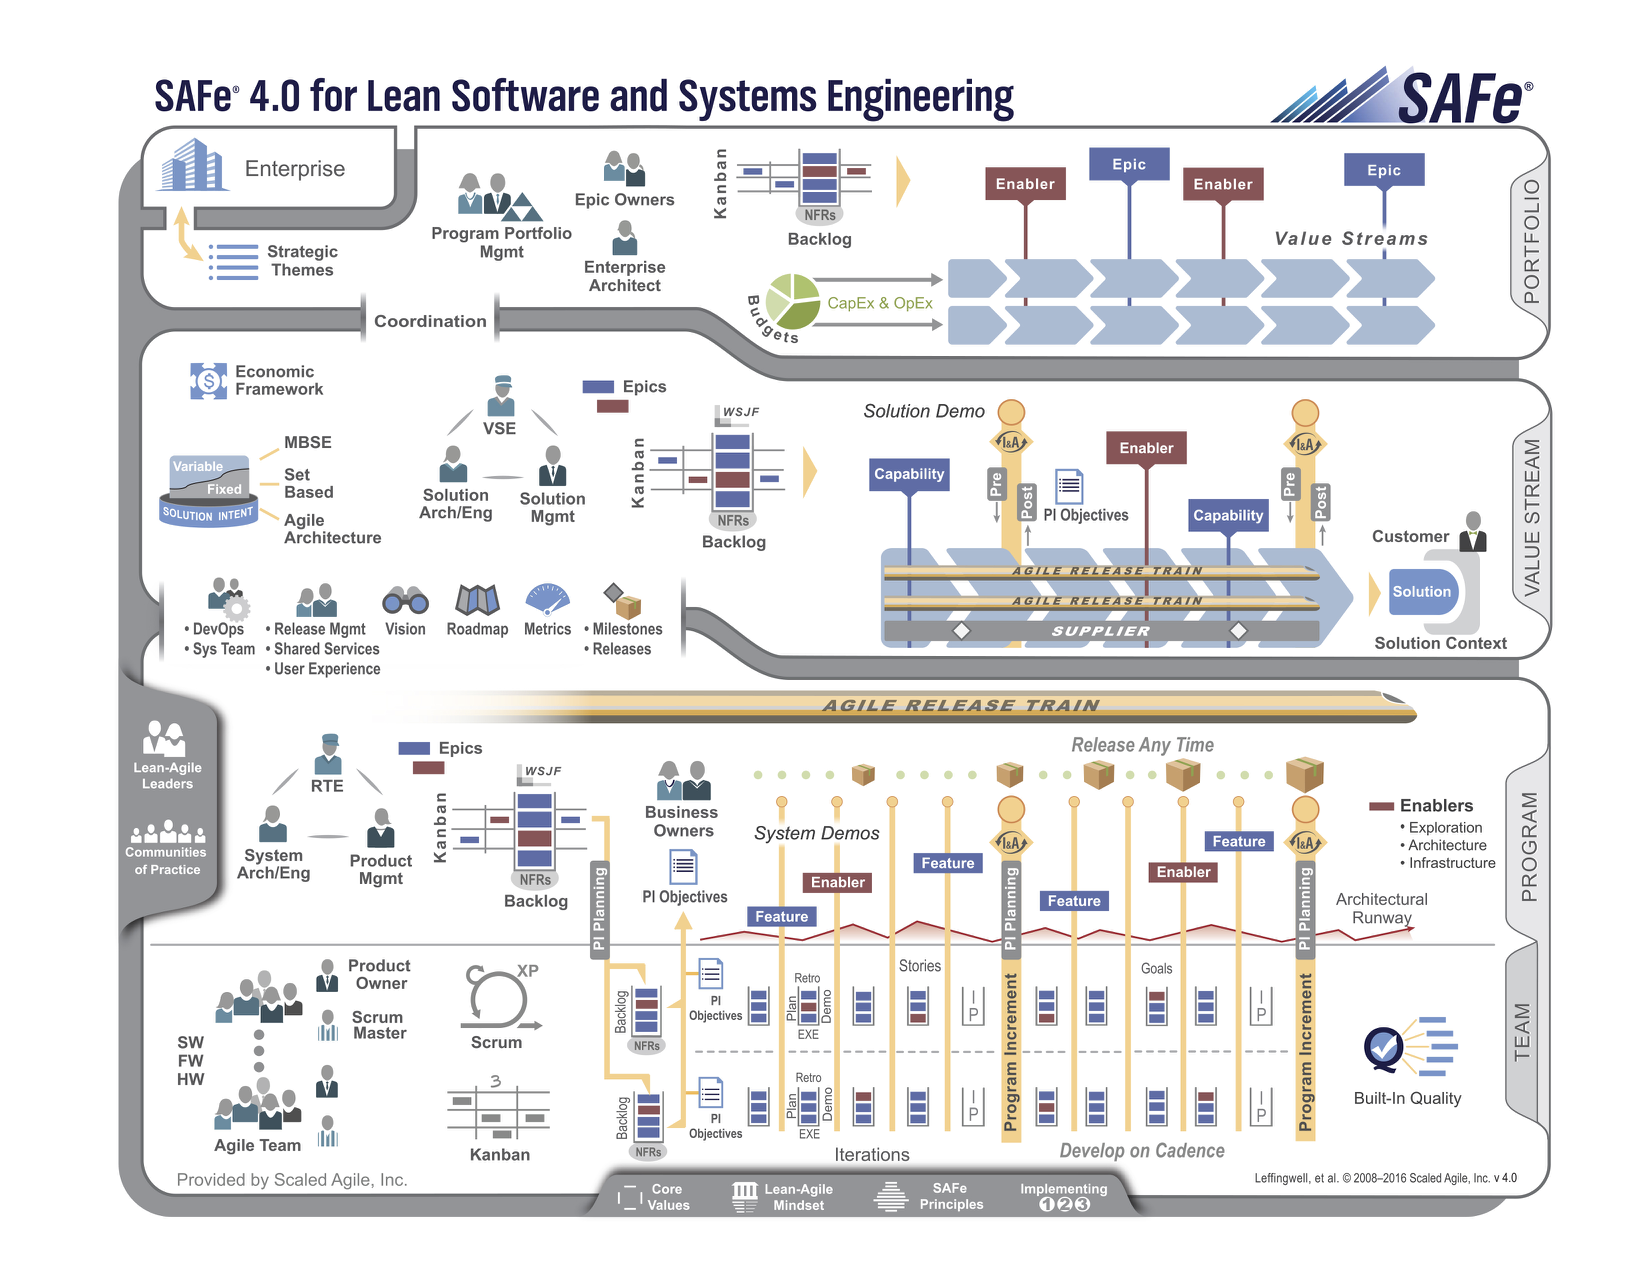
\includegraphics[scale=0.5]{figuras/SAFe_big_picture}
    \caption[Big Picture do SAFe <>]{Big Picture do SAFe. \footnotemark}
    \label{big-picture-safe}
  \end{figure}
    \footnotetext{Fonte: \cite{safe}}
  \newpage

  \section{RUP}
O Rational Unified Process (RUP) é um processo de Engenharia de Software iterativo e incremental desenvolvido no final dos anos 90. Fornece uma abordagem disciplinada para se delegar tarefas e responsabilidades dentro de uma organização de desenvolvimento, cujo objetivo é assegurar a produção de \textit{software} de alta qualidade dentro de prazos e orçamentos previsíveis e controlados~\cite{kruchten}.

É considerado um processo tradicional de sucesso para lidar com aplicações de larga escala robustas, escaláveis e extensíveis, por isso foi o primeiro processo largamente adotado que reconheceu a necessidade de estender a área de abrangência das atividades que ocorriam nas fases de iniciação, elaboração, construção e transição durante o ciclo de vida~\cite{deanleffingwell}.

    \begin{figure}[!htbp]
    \centering
    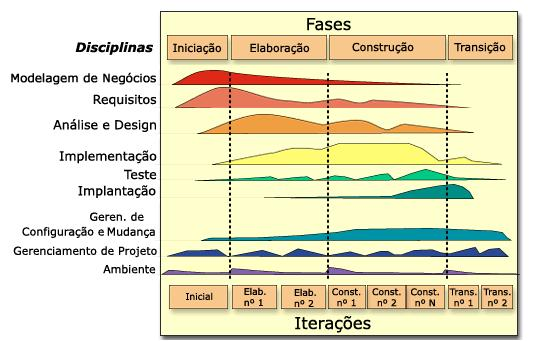
\includegraphics[scale=3.0]{figuras/Fases_do_RUP_-_portugues}
    \caption[Fases do RUP]{Fases do RUP. \footnotemark}
    \label{fases-rup}
  \end{figure}
  \footnotetext{Fonte: \cite{rup}}
Este processo é abstraído em duas dimensões estruturais:
\begin{itemize}
\item O eixo horizontal representa o tempo dividido nas fases do processo 	(Iniciação, Elaboração, Construção e Transição). Diz 	respeito ao aspecto dinâmico do processo quando ele é aprovado.
\item O eixo vertical representa os aspectos estáticos do processo, as 	disciplinas, fluxos de trabalho, papéis, atividades e artefatos. 	[WTHREEX]
\end{itemize}

Segundo Sommerville, o RUP aborda as melhores práticas verificadas empiricamente ao longo do tempo para o desenvolvimento de software~\cite{sommerville}:

\begin{description}
\item[1. Desenvolver o software iterativamente:] Trabalhar com incrementos de \textit{software} com baseando-se na atribuição de prioridades para determinadas funcionalidades, entregando o mais cedo possível as características de sistema de maior prioridade no processo de desenvolvimento.
\item[2. Gerenciar requisitos:] manter um processo de documentação sistemática dos requisitos do cliente e gerenciar mudanças nesses requisitos, avaliando o impacto geral dessas alterações antes de aceitá-las.
\item[3. Arquiteturas baseadas em componentes:] Estruturar a arquitetura do sistema com componentes, modularizando e reduzindo a quantidade de software a ser desenvolvido e, consequentemente, diminuindo custos e riscos.
\item[4. Modelar software visualmente:] usar modelos gráficos de UML para apresentar as visões estática e dinâmica do \textit{software}, de modo a alinhar a visão dos envolvidos no projeto, reduzindo os riscos de uma solução que não seja condizente com o real problema.
\item[5. Verificar a qualidade do software:] garantir que o software atenda aos padrões de qualidade exigidos pelo mercado de acordo com a organização.
\item[6. Gerenciar as mudanças do software:] controlar as mudanças no \textit{software}, fazendo o uso de procedimentos e ferramentas de gerenciamento de configuração de modo a reduzir os riscos e manter a viabilidade da construção da aplicação dentro dos prazos e custos estabelecidos.
\end{description}

Tomando como base essas características, a aplicabilidade do RUP como processo base para o suporte de novos projetos pode ser conseguida de várias maneiras. Uma delas seria usar o RUP à risca, isto é, seguir todos os métodos e processos única e exclusivamente como são propostos. O ponto positivo desta abordagem é que se nada é alterado, o RUP é essencialmente completo e detalhado. Entratanto, existe um preço muito alto a ser pago, este diz respeito à sua complexidade por vezes desnecessária. Esta abordagem automaticamente aumentaria os custos em treinamentos, projetos piloto, e algumas atividades, sendo este um fator chave para inviabilizar a aplicação pura do RUP em uma série de projetos.

Outra maneira seria a adoção de outro modelo de processo mais simples que utiliza parcialmente o material do RUP como fonte de referência complementar, adequando o processo tradicional ao escopo do projeto. Desse modo, o RUP pode fazer parte de uma escolha viável para pequenos projetos e equipes assim como a apresentada neste documento.

  \section{Modelo de maturidade}
  Os modelos de maturidade de processos são um referencial usado para:
\begin{itemize}
\item Avaliar a capacidade de processos na realização de seus objetivos
\item Localizar oportunidades de melhoria de produtividade e qualidade e de reducão de custos
\item Planejar e monitorar as ações de melhoria contínua dos processos empresariais
\end{itemize}

  \subsection{Modelo CMMI(Capability Maturity Model Integration)}
  O CMMI é um modelo de referência que define práticas sejam elas genéricas ou específicas necessárias para o desenvolvimento e avaliação de maturidade no desenvolvimento de softwares em uma organização. As práticas que são abordadas neste modelo são: gerenciamento de requisitos, manipulação de riscos, medição de desempenho, planejamento de trabalho, tomada de decisão, entre outros. O modelo CMMI não pode ser considerado uma metodologia, pois não orienta como deve ser feito, e sim o que deve ser feito. Esse modelo foi desenvolvido pelo SEI(Software Engineering Institute) da Universidade Carnegie Mellon. É uma evolução do CMM, que foi baseado em algumas das ideias mais importantes dos movimentos de qualidade industrial das últimas décadas.
No CMMI uma organização opta por duas representações para a melhoria dos seus processos: Por estágios e contínua.\cite{modelosmaturidade}
  \begin{figure}[!htbp]
    \centering
    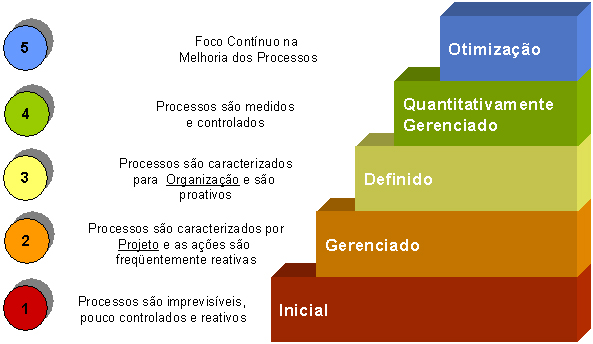
\includegraphics[scale=0.5]{figuras/cinco-niveis-maturidade-cmmi}
    \caption[Níveis de Maturidade]{Níveis de Maturidade. \footnotemark}
    \label{cinco-niveis-maturidade-cmmi}
  \end{figure}
    \footnotetext{Fonte: \cite{cmmi}}

  \subsection{Modelo MPS-BR (Melhoria de Processo do Software Brasileiro)} \label{mps-br}
MPS-BR significa Melhoria de Processo do Software Brasileiro, criado pelo Softex e patrocinado pelo MCT. O modelo de maturidade de processos e desenvolvimento de software conhecido como CMMI-DEV foi adaptado para empresas brasileiras, em especial para micro, pequenas e médias empresas, dando origem ao MPS-BR. Essa adaptação foi necessária por que o CMMI-DEV prevê o amadurecimento dos processos em apenas cinco níveis.\cite{modelosmaturidade}

E com o passar do tempo percebeu-se a necessidade de uma funcionalidade mais gradual aqui no Brasil, por isso foi quebrado os cinco níveis do CMMI-DEV em sete, com vemos na figura a seguir:
  \begin{figure}[!htbp]
    \centering
    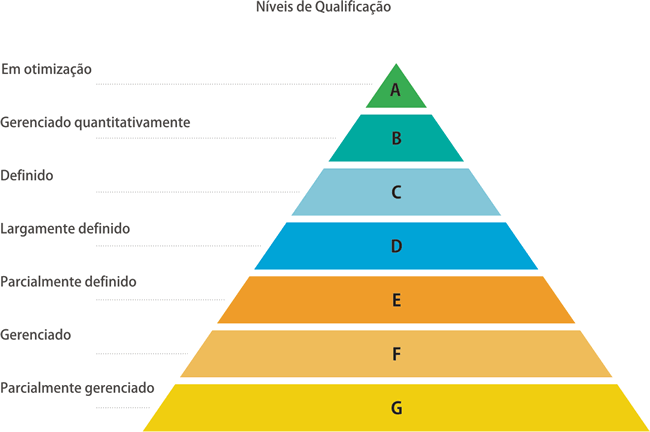
\includegraphics[scale=0.5]{figuras/650x432xniveis_de_qualificacao}
    \caption[Níveis de Maturidade do MPS-Br]{Adaptada, níveis de Maturidade do MPS-Br. \footnotemark}
    \label{niveis-maturidade-mps-br}
  \end{figure}
    \footnotetext{Fonte: \cite{mps-br}}
  
Como ilustrado na imagem, o MPS-Br possui possui uma divisão semelhante ao CMMI, entretando o mesmo encontra-se dividido nos níveis constituintes do A ao G, sendo o nível A o mais alto qualitativamente e o G o nível inicial(MPS de Software, São Paulo: SOFTEX, 2012).	
\begin{description}
\item[A.] Em otimização
\item[B.] Gerenciado quantitativamente
\item[C.] Definido
\item[D.] Largamente definido
\item[E.] Parcialmente definido
\item[F.] Gerenciado
\item[G.] Parcialmente gerenciado	
\end{description}			

Os processos referentes a engenharia de requisitos estão descritos no níveis, G e D, correspondentes aos processos de "Gerência de requisitos respectivamente" e "Desenvolvimento de requisitos".

\textbf{Gerência de requisitos}

Como o nome já diz, tem como objetivo gerenciar os requisitos do produto e dos componentes do produto/projeto, além de identificar inconsistências entre requisitos, planos e produtos de trabalho do projeto.

\textbf{Resultados esperados:}
\begin{itemize}
\item \textbf{GRE 1} - O entendimento dos requisitos é obtido junto aos fornecedores de requisitos.
\item \textbf{GRE 2} - Os requisitos são avaliados com base em critérios e objetivos e um comprometimento da equipe técnica com estes requisitos é obtido.
\item \textbf{GRE 3} - A rastreabilidade bidirecional entre os requisitos e os produtos de trabalho é estabelecida e mantida.
\item \textbf{GRE 4} - Revisões em planos e produtos de trabalho do projeto são realizadas visando identificar e corrigir inconsistências em relação aos requisitos.
\item \textbf{GRE 5} - Mudanças nos requisitos são gerenciadas ao longo do projeto.
\end{itemize}

\textbf{Desenvolvimento de requisitos:}
Visa definir os requisitos do cliente, do produto e dos componentes do produto.

\textbf{Resultados esperados:}
\begin{itemize}
\item \textbf{DRE 1} - As necessidades, expectativas e restrições do cliente, tanto do produto quanto de suas interfaces, são identificadas.
\item \textbf{DRE 2} - Um conjunto definido de requisitos do cliente é especificado e priorizado a partir das necessidades, expectativas e restrições identificadas.
\item \textbf{DRE 3} - Um conjunto de requisitos funcionais e não-funcionais, do produto que descrevem a solução do problema a ser resolvido, é definido e mantido a partir dos requisitos do cliente.
\item \textbf{DRE 4} - Os requisitos funcionais e não-funcionais de cada componente do produto são refinados, elaborados e alocados.
\item \textbf{DRE 5} - Interfaces internas e externas do produto e de cada componente do produto são definidas.
\item \textbf{DRE 6} - Conceitos operacionais e cenários são desenvolvidos.
\end{itemize}
  \section{Contexto dentro do projeto}
Neste projeto foi definida a utilização do modelo MPS-Br, levando em conta que ele é bem semelhante ao modelo CMMI e vai possibilitar a produção de resultados parecidos. Também foram observados outros critérios para a definição do modelo a ser utilizado.

Segundo a SOFTEX, mantenedora do MPS.BR, grande parte do modelo de maturidade é mantido em parte por instituições de ensino, isto garante uma integração permanente do modelo com o meio acadêmico, possibilitando a absorção dos avanços obtidos em pesquisas. É facilitada assim a aplicação do modelo em projetos desenvolvidos na academia, que, segundo vários especialistas, está alguns anos na frente do mercado. 

Assim, o MPS-Br foi a primeira opção destacada pelo grupo. Atentando-se também ao fato de ser um modelo que se adapta a realidade do desenvolvimento de software no Brasil. Como dito na seção \ref{mps-br}, o modelo foi pensado para ser utilizado no contexto de micro, pequenas e médias empresas, o que é virtualmente a característica da presente equipe, uma vez que o nosso cliente é uma empresa júnior de engenharia eletrônica. Outro fator que vale a pena destacar é o fato de que o MPS-Br possui uma maior divisão de níveis de maturidade, o que torna o processo suscetível a atingir níveis maiores de maturidade com maior simplicidade já que, essa característica de possuir mais níveis, confere um menor número de processos em cada nível, comparando-se com o CMMI.
\section{Mapeamento do contexto e abordagem}
Levando em consideração as diferentes abordagens que foram apresentadas, algumas características foram mapeadas de forma a elucidar a melhor escolha de processo a se fazer. Essas características estão relacionadas ao contexto da equipe, escopo do projeto, cliente e ambiente de trabalho.

\begin{itemize}
\item \textbf{A} - A pequena quantidade de pessoas na equipe, quatro membros, facilita seu auto gerenciamento.
\item \textbf{B} - O impacto resultante de uma atribuição funcional específica para um dos membros é extremamente relevante para uma equipe de tamanho reduzido e pode influenciar diretamente o sucesso do projeto principalmente em relação aos prazos a serem cumpridos.
\item \textbf{C} - Todos os membros da equipe já participaram de projetos os quais se utilizava uma abordagem ágil. Alguns nunca trabalharam de forma incisiva com metodologias tradicionais.
\item \textbf{D} - A equipe tem disponibilidade para se encontrar pelo menos 3 vezes na semana presencialmente e 7 vezes através de ferramentas com Google Hangouts.
\item \textbf{E} - O cliente possui grande disponibilidade para ser encontrado próximo ao nosso ambiente de trabalho. Seu representante, inclusive, participa de algumas disciplinas do curso de Engenharia de Software da Universidade de Brasília com os próprios membros da equipe.
\item \textbf{F} - A Empresa Júnior Eletronjun, apesar de ser a mais antiga das empresas juniores da Faculdade do Gama, ainda se encontra em processos de construção, estabelecimento no mercado, levantamento de cliente. Sendo assim, o escopo do projeto pode sofrer alterações substanciais no decorrer do desenvolvimento.
\item \textbf{G} - Um dos membros da presente equipe já trabalho na equipe de T.I e Marketing da Eletronjun nessa mesma gestão, o que favorece o diálogo e o reconhecimento do cliente por parte dos membros do grupo.
\item \textbf{H} - O projeto possui um tempo relativamente curto para ser implementado, com uma expectativa de 45 dias.
\item \textbf{I} - Os membros da equipe já se conheciam antes e trabalharam juntos, não todos, mas em parte, em outros projetos de disciplinas no curso de Engenharia de Software.
\end{itemize}			

  \section{Justificativa}
Conforme a seção anterior, a metodologia escolhida para a confecção deste trabalho foi uma abordagem ágil, fundamentada no SAFe.

Esta escolha foi baseada nas características da equipe, do projeto e do cliente, que automaticamente encontraram maior correspondência adaptativa em uma abordagem que segue os princípios do desenvolvimento ágil.

“A engenharia de software ágil combina filosofia com um conjunto de princípios de desenvolvimento. A filosofia defende a satisfação do cliente e a entrega de incremental prévio; equipes de projetos pequenas e altamente motivadas; métodos informais; artefatos de engenharia de software mínimos e, acima de tudo, simplicidade no desenvolvimento geral. Os princípios de desenvolvimento priorizam a entrega mais que a análise e projeto, embora essas atividades não sejam desencorajadas; também priorizam a comunicação ativa e contínua entre desenvolvedores e clientes”. (PRESSMAN, 2012)

Um outro fator muito importante para a escolha desta metodologia foi o prévio relacionamento que um dos membros do grupo tinha com o nosso cliente, uma vez que o mesmo já havia trabalhado na empresa, além de conhecer a sua estrutura, seus processos e parte da equipe. Isso tornou o processo mais fluido, uma vez que não tivemos a necessidade de fazer uma pesquisa minuciosa a fim de conhecer melhor a empresa.

Segundo Mike Cohn, autor do livro Desenvolvimento de Software com Scrum, uma equipe pequena consegue eficientemente uma ótima interação, facilitando o processo de desenvolvimento de um software, mas há um grande problema: como a equipe é pequena, qualquer perda ou comprometimento de um membro é potencialmente danoso ao projeto como um todo. Para que isso seja evitado, não deve haver grande especialização na equipe, ou seja, todos devem ser responsáveis pelo projeto, sem papéis fixos e inflexíveis, o que torna a equipe dinâmica e faz com que a metodologia se adapte ao escopo do problema.
